\subsubsection{Correlation Traps}
%\paragraph{Correlation Traps.}
\label{sxn:Traps}

The first way we identify $\mathbf{W}$ as \ATypical is when it has an anomalously large mean $(\bar{\WMAT})$;
detecting this in general, however, requires more than just examining which elements $W_{i,j}$ are
anomalously large.
\michaeladdressed{Ugh.}

The \HTSR \Phenomenology states that NNs generalize better when their layers ESDs are more HT---precisely because the 
tail eigenvalues arise from correlations in the weight matrices.
So one way is to identify \emph{atypicality} is to look for  large eigenvalues that
do not arise from correlations in $\mathbf{X}$,
but, rather, from one or a few spuriously large matrix elements $W_{i,j}$ and/or rank-1 perturbations in $\mathbf{W}$.
\michaeladdressed{Do we have an example of this.}
We call these eigenvalues  \CorrelationTraps, denoted by $\lambda_{trap}$
(i.e., see Section~\ref{sxn:empirical-correlation_trap}).

Indeed, if we randomize $\mathbf{W}$ elementwise, i.e $\mathbf{W}\rightarrow\mathbf{W}^{rand}$, we
expect the $W^{rand}_{i,j}$ matrix elements to be i.i.d and with a small mean
(unless something odd happens during SGD training).
Likewise, we expect the singular values of $\WMAT^{rand}$ to follow the MP distribution, to within
finite-size / TW fluctuations.
If we observe an eigenvalue $\lambda_{trap}$ extending beyond the MP bulk region, $\lambda_{trap}>\lambda^{+}_{bulk}$,
then the mean $W_{i,j}$ matrix element will also be anomalously large,
and we can identify $\mathbf{W}$ as \ATypical.
We must be careful, however, as we do not fully understand the origin of these atypicalities
and do not claim that every one is associated with suboptimal generalization.

%One way would be to look for  $\mathbf{W}$ is HT elementwise such that the $W_{i,j}$ are Pareto distributed,
%with a PL exponent less tha $1.0$;  in this case, the mean is not well-defined .
%This is not observed, however, as for most well trained NNs,
%the $W_{i,i}$ are best fit to a Laplacian distribution, so the tail decays exponentially.

%Never-the-less, we do frequently observe cases in large, pretrained models
%4%where the layer  $\mathbf{W}$  exhbits  an anomalously large mean caused
%ne or a few anmoloulsy large $W_{i,i}$ and/or rank-1 perturbatons,
%which are manifest as spuriously large eigenvalues.
%The presence of such anomalies in a weight matrix suggests
%that the matrix is  \ATypical; we call these anomalies \CorrelationTraps.

By a \emph{\CorrelationTrap}, we mean that some anomaly in the training of $\mathbf{W}$ resulted
in one or more spuriously large eigenvalues $\lambda_{trap}$ in $W^{rand}$,
and that  whatever caused them also may, in some pronounced cases, tend
to ``trap the correlations in $\mathbf{X}$ itself,
preventing them from coalescing into a well defined PL Heavy Tail,
or otherwise distorting the ESD.
Whether they are a signature of training gone wrong, or whether they distort the dynamics of the tail correlations 
simply by being there, \CorrelationTraps can be expected to alter the shape of the ESD,
reducing the quality of the PL fits, and sometimes producing spurious $\alpha$ values.

Why would such anomalies  occur in a NN?
It is conceivable that SGD will, when it fails to find usable correlations, instead
produce spurious
correlations in the form of large elements and/or rank-1 perturbations.
Also, the matrix itself may simply undergo an innocuous  mean-shift because the
mean is not explicitly controlled during training. Here,  mean-recentering may be beneficial.
\footnote{Similarly, when training NNs, frequently the weight matrices~\cite{baskin2021} or activations~\cite{choi2018_TR}
may need to be clipped during training to ensure good results.}

We will see, below in Section~\ref{sxn:empirical}, that we can induce a \CorrelationTrap both by shrinking the batch 
size, or, equivalently, increasing the learning rate, and that this is associated with degraded model performance
and small $\alpha$.
We seek to identify specific ways of identifying such traps because we 
reason that the self-organization of correlations may be disrupted by the presence of foreign large eigenvalues – or that failed learning may produce them as a by-product.


%Using the \HTSR \Phenomenology, we can classify (some of) the features of the weight matrix itself
%that seem to arise from suboptimal training and that make an ESD more HT than desired and/or
%deformm the empirical ESD $\rho^{emp}(\lambda)$.
%We call these \SCALE~anomalies.
%Such \SCALE~anomalies may arise when training with an excessively small batch size (see Section~\ref{sxn:empirical}), 
%an unusually large learning rate, or just when the layer regularization fails.
%\michael{Why call them scale anomalies, i.e., why introduce a new term.}
%Indeed, when training NNs, frequently the weight matrices may need to be clipped during
%training to ensure good results. 
%\michael{Who does that clipping.}
%The \HTSR \Phenomenology also suggests that mean-recentering may be beneficial as well.
%In these situations, the PL fits may show spuriously small PL exponents $\alpha$, and this
%is sometimes reflected, detectable, and even correctable.
%We call these \CorrelationTraps; they
%alter the shape of the ESD, reducing the quality of the PL fits,
%making $\alpha$ smaller than expected.


\paragraph{Detecting Correlation Traps with \RMT.}

RMT suggests that when a matrix $\mathbf{W}$ has unusually large elements $W_{ij}$, then the ESD will have one or more large eigenvalues $\lambda$ lying outside the bulk edge $\lambda^{+}_{bulk}$ of the ESD, as predicted by MP theory. 
One can detect these so-called \CorrelationTraps in a weight matrix $\mathbf{W}$ by performing the following:
\begin{enumerate}
\item randomize $\mathbf{W}$ element-wise to obtain $\mathbf{W}^{rand}$;
\item compute the ESD for $\mathbf{W}^{rand}$; and
\item look for large eigenvalues $\lambda_{trap}\gg\lambda^{+}_{bulk}$.
\end{enumerate}
\WW~looks for \CorrelationTraps ($\lambda_{trap}$) in the ESD of the randomized $\mathbf{W}^{rand}$, that are larger than 
$ \lambda_{trap}>\lambda^{bulk}_{+}+\Delta_{TW} , $ 
where 
$\lambda_{bulk}$ is the MP bulk edge $\Delta_{TW}$ are the associated finite-size Tracy Widom (TW) fluctuations. 
This procedure detects \emph{any} anomaly in the matrix weights that produces a spuriously large eigenvalues. 
It is implemented in \WW (using the randomize option), which was used to generate the plots in Figure~\ref{fig:scale-shape}.

\begin{figure}[h]
    \centering
    \subfigure[Well-formed ESD]{ 
      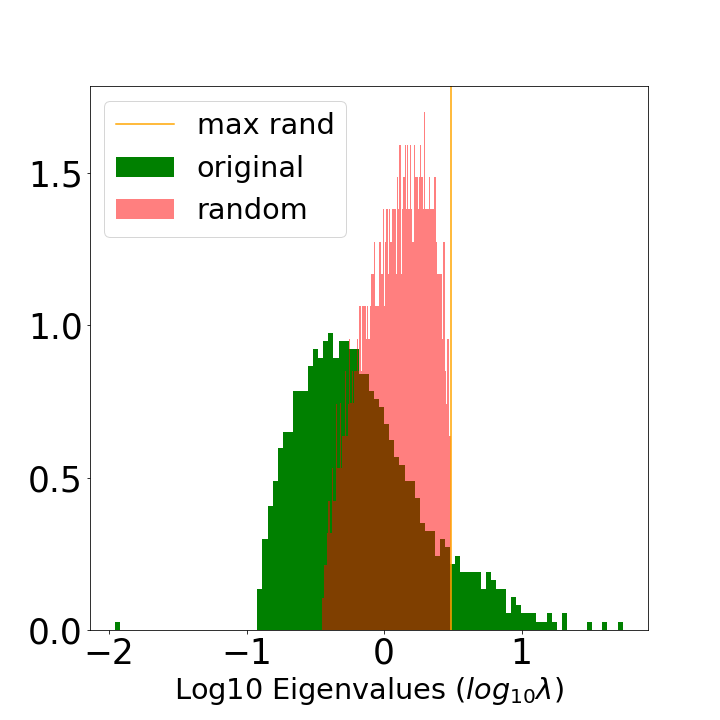
\includegraphics[width=4cm]{./img/shape-scale-a.png}
      \label{fig:scale-shape-a}
    }                               
    \subfigure[ESD with \CorrelationTrap]{                   
      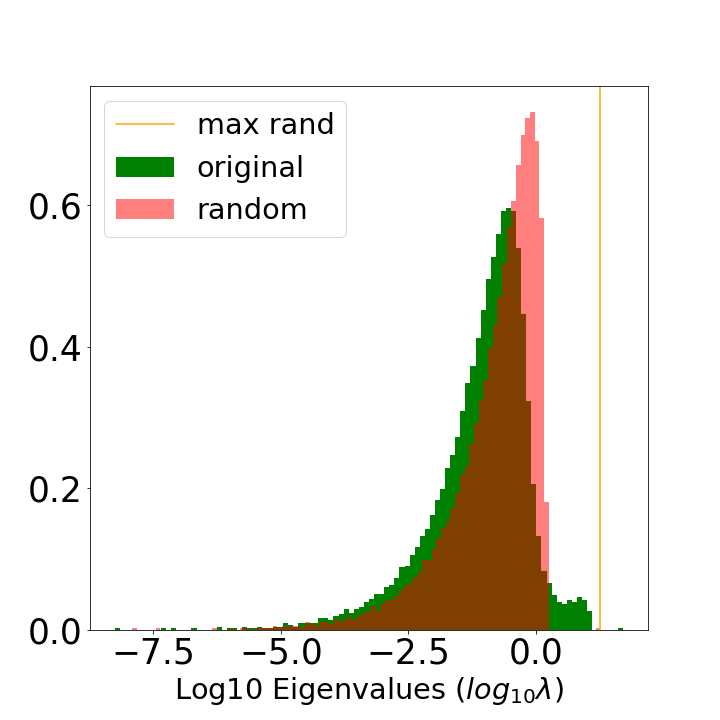
\includegraphics[width=4cm]{./img/shape-scale-b.png}
      \label{fig:scale-shape-b}                                                                                                      
    }                                                                                                                            
    \caption{Comparison of a well-formed, Heavy-Tailed ESD (a) to one with a Correlation Trap (b), in the VGG16 model (FC2 layer)}
  \label{fig:scale-shape}                                                                                                      
\end{figure}

See Figure~\ref{fig:scale-shape-a}, which displays the (log)-ESD of a \Typical SOTA NN layer $\mathbf{X}$ (green), i.e., on a log-linear scale, along with the (log)-ESD of that layer after randomizing it element-wise (red).
The two ESDs differ substantially:
the ESD of the original weight matrix  $\mathbf{W}$ (green) is very HT, whereas 
the ESD of the randomized weight matrix  $\mathbf{W}^{rand}$ (red) is a MP (and as predicted by the MP \RMT).
The orange line corresponds to the maximum eigenvalue of the randomized ESD.
Note that it is at the MP bulk edge of the red plot, indicating that this ESD is not affected by unusually large elements or other weight anomalies.
Here, we say that the ESD of $\mathbf{X}$ is HT, and that $\mathbf{W}$ is not HT element-wise.
\HTSR says this layer is well-trained.

Contrast this with Figure~\ref{fig:scale-shape-b}, which displays the (log)-ESD of a NN layer with a \CorrelationTrap.
The ESD of $\mathbf{X}$ (green) is weakly HT, but it looks nothing like the ESD in Figure~\ref{fig:scale-shape-a}.
In fact, it looks very much like the ESD of the randomized weight matrix  $\mathbf{W}^{rand}$ (red), except for a small shelf on the right. 
The orange line again corresponds to the maximum eigenvalue of the randomized ESD, and this is just past this shelf.
Relative to the randomized ESD, this line depicts (an) unusually large element(s)---or, equivalently, a rank-1 perturbation of $\mathbf{W}^{rand}$.
By a \CorrelationTrap, we mean that some anomaly in the elements of $\mathbf{W}$ tends to ``trap'' the ESD of $\mathbf{X}$, concentrating the correlations in $\mathbf{X}$ into the small shelf of density around the orange line. 
%\michael{That sentence should probably be above.}
\HTSR says this layer is not well-trained because it does not have a good PL fit.

%We will see, below in Section~\ref{sxn:empirical}, that we can induce a \CorrelationTrap by shrinking the batch size, and that this is associated with a degradation in model performance (%as well as spuriously low PL exponent $\alpha$). 
%\michael{This should be elsewhere.}


%\paragraph{Correcting for \SCALE Anomalies with \ALPHAHAT}
%\subsubsection{Correcting for Scale Anomalies with \ALPHAHAT}

%\nred{repetitive ?}
%  \CorrelationTraps are a kind of \SCALE anamoly;by this we mean when the layer weight matrix $\mathbf{W}$
%  and/or the randomized  $\mathbf{W}^{rand}$ has one or more unusually large eigenvalues $\lambda$.
%  In the case of a scale anamoly, the simple PL \ALPHA metric may not correlate well with the test accuracy or other measures
%  of model quality because such scale anomalies may make it difficult to get a good PL fit of $\alpha$.
%  In some very hard cases, the layer ESD $\rho_{emp}(\lambda)$ may be significantly deformed from a well
%  behaved PL or TPL distribution (as in Fig.~\ref{fig:scale-shape-b}.  In these cases, the \ALPHAHAT
%  metric can frequently compensate.  This is seen in Section~\ref{sxn:empirical} \nred{see github issue 46}

 



